\section{Automatic Speech Recognition (ASR)}
\begin{frame}{}
    \LARGE \textbf{Automatic Speech Recognition (ASR)}
\end{frame}

\begin{frame}[allowframebreaks]{Automatic Speech Recognition (ASR)}

\begin{itemize}
    \item Automatic Speech Recognition converts spoken language (audio) into written text.  
    \item Example:  
    \[
        \resizebox{\linewidth}{!}{$
        \text{Audio: ``Hey computer, what's the weather?''} \rightarrow \text{Text: ``hey computer what's the weather''}
        $}
    \]

    \item How it works (high-level pipeline):
    \begin{itemize}
        \item Extract features from audio (e.g., log-Mel spectrograms, MFCCs).
        \item Pass features through an \textbf{acoustic model} to map audio patterns to phonemes or subword units.
        \item Use a \textbf{language model} to predict the most probable word sequences.
        \item Decode the combined outputs into final text.
    \end{itemize}
\framebreak
    \item Why ASR is important:
    \begin{itemize}
        \item Enables natural language interaction with computers (voice assistants).  
        \item Facilitates transcription, accessibility, and spoken-input NLP applications.
    \end{itemize}
\end{itemize}

\framebreak

\begin{figure}
    \centering
    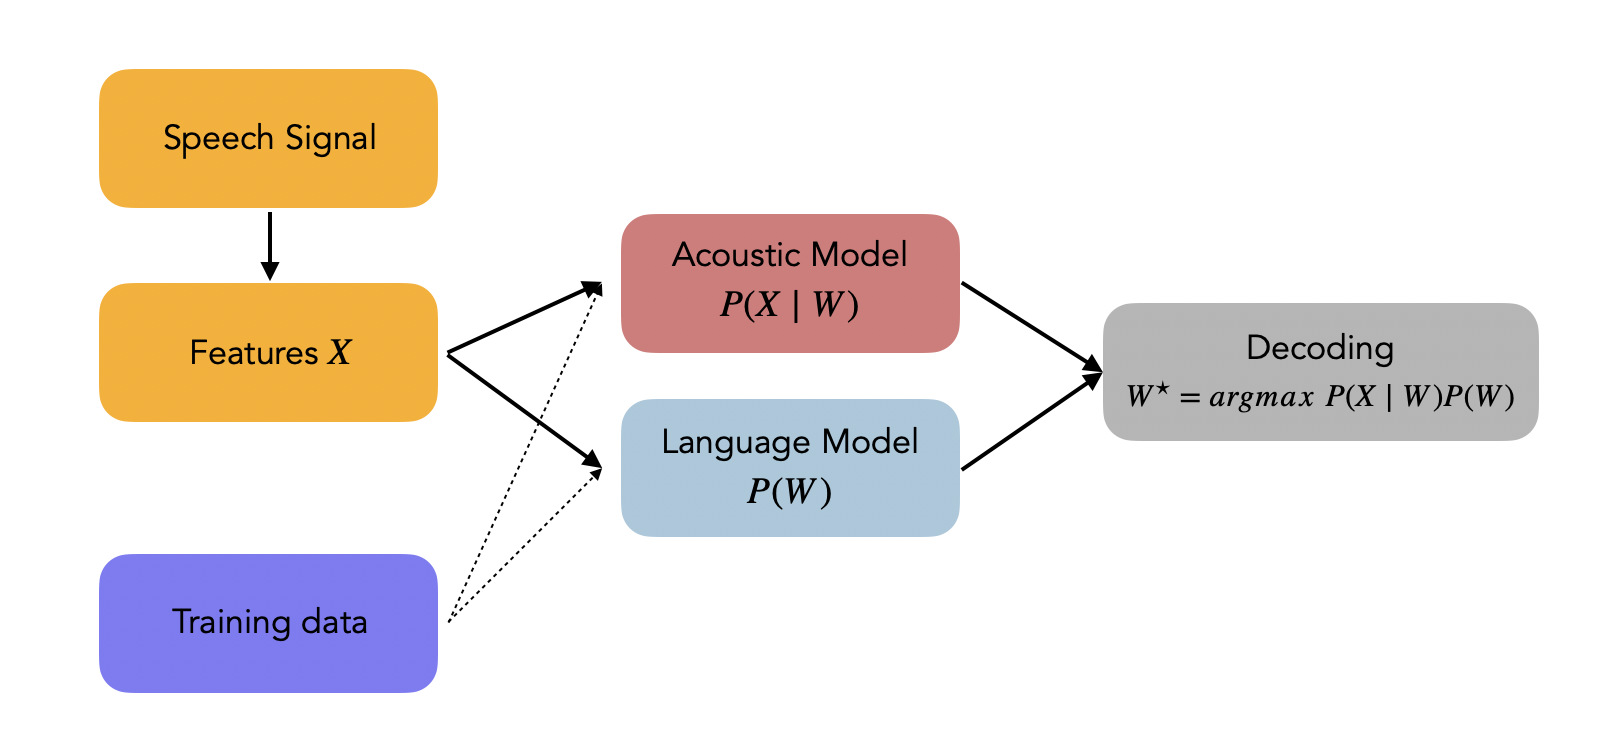
\includegraphics[width=\textwidth,height=0.6\textheight,keepaspectratio]{images/audio-nlp-eval/asr-diagram.png}
    \caption*{Statistical historical approach to ASR.\\
    {\scriptsize Source: M.~Fabien, ``Introduction to Automatic Speech Recognition (ASR),'' \url{https://maelfabien.github.io/machinelearning/speech_reco/}}}
\end{figure}

\end{frame}


\begin{frame}[allowframebreaks]{Traditional ASR Pipeline}

\begin{itemize}
    \item Traditional ASR systems were built as modular pipelines with interpretable components.  
    \item Main components:
    \begin{itemize}
        \item \textbf{Acoustic model:} estimates $P(x \mid \text{phones})$, mapping audio features to phonetic units.
        \item \textbf{Pronunciation dictionary:} converts phones to words.
        \item \textbf{Language model:} estimates $P(\text{words})$, guiding likely word sequences.
        \item \textbf{Decoder:} searches for the most probable word sequence given the acoustic and language models.
    \end{itemize}

    \item Mathematical formulation:
    \[
        \hat{W} = \arg\max_W P(W \mid X) = \arg\max_W P(X \mid W) \, P(W)
    \]
    where $W$ = word sequence, $X$ = extracted audio features.

    \item Why this approach worked:
    \begin{itemize}
        \item Easier to engineer and understand.
        \item Interpretable: each module can be improved independently.
    \end{itemize}

    \item Limitations:
    \begin{itemize}
        \item Complex, hand-crafted system.
        \item Errors can propagate through the pipeline.
    \end{itemize}
\end{itemize}

\end{frame}


\begin{frame}[allowframebreaks]{End-to-End ASR}

\begin{itemize}
    \item Modern ASR systems often replace traditional modular pipelines with \textbf{neural sequence-to-sequence models}, directly mapping audio features to text.  

    \item Popular approaches:
    \begin{itemize}
        \item \textbf{CTC (Connectionist Temporal Classification)} – handles variable-length alignments.
        \item \textbf{Attention-based encoder-decoder} – learns soft alignments between input frames and output tokens.
        \item \textbf{Transducer models} – integrate CTC-style alignment with recurrent decoding.
    \end{itemize}

    \item Advantages:
    \begin{itemize}
        \item Minimal handcrafting of features or components.
        \item Often achieves better accuracy when trained on large datasets.
    \end{itemize}

    \item Each approach solves the same problem, that the audio has far more frames than the transcript has tokens, in a different way. We take them one at a time in the sections that follow.

    \item Reference: Hannun, ``Sequence Modeling With CTC'', Distill, 2017. \url{https://distill.pub/2017/ctc/}
\end{itemize}

\end{frame}


\begin{frame}[allowframebreaks]{Whisper (OpenAI)}

\begin{itemize}
    \item Whisper is a state-of-the-art, multilingual ASR model developed by OpenAI.  

    \item Key architecture:
    \begin{itemize}
        \item Encoder-decoder transformer.
        \item Trained on 680,000 hours of \textbf{weakly supervised} audio: transcripts scraped from the web and paired with audio, not annotated for the task. 117,000 of those hours are non-English.
        \item Takes 80-channel log-Mel spectrograms as input (25~ms window, 10~ms hop).
    \end{itemize}

    \item Advantages:
    \begin{itemize}
        \item Robust to different accents and noisy environments.
        \item Supports multitask learning: ASR and optional translation.
    \end{itemize}

    \item Example use case:
    \begin{itemize}
        \item Spoken French: ``Je parle français'' → can output English translation.
    \end{itemize}
\end{itemize}

\begin{figure}
    \centering
    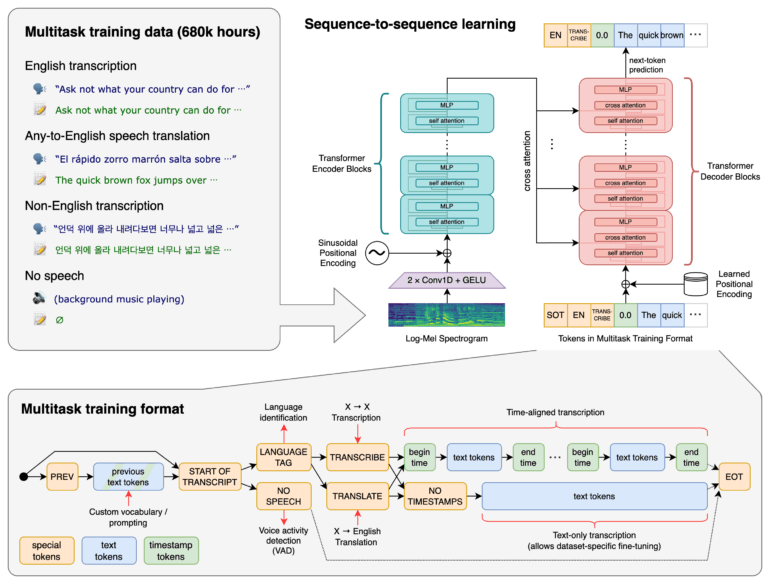
\includegraphics[width=\textwidth,height=0.8\textheight,keepaspectratio]{images/audio-nlp-eval/whisper.png}
    \caption*{\scriptsize Source: Radford et al., ``Robust Speech Recognition via Large-Scale Weak Supervision'', 2022, Fig.~1.}
\end{figure}

\end{frame}


\begin{frame}[allowframebreaks]{Conformer (Conv + Transformer)}

\begin{itemize}
    \item Conformer is a hybrid neural model that combines \textbf{convolutions} and \textbf{transformers} to process speech effectively.  

    \item Core components:
    \begin{itemize}
        \item \textbf{Convolution:} captures local structures and fine-grained temporal patterns in audio.
        \item \textbf{Self-attention:} captures global context and long-range dependencies.
    \end{itemize}

    \item Achievements:
    \begin{itemize}
        \item Was state of the art on LibriSpeech when published: $2.1\%$ / $4.3\%$ WER on test-clean / test-other without a language model, and $1.9\%$ / $3.9\%$ with an external LM (Conformer~(L), 118.8M parameters).
        \item Balances efficiency and accuracy better than pure transformer or CNN models alone: a 10.3M-parameter Conformer~(S) still reaches $2.7\%$ / $6.3\%$.
    \end{itemize}

    \item Block equations: the four modules are applied \emph{in sequence}, each as a pre-norm residual, with the two feed-forward modules half-weighted and sandwiching the attention and convolution pair:
    \begin{align*}
        \tilde{x} &= x + \tfrac{1}{2}\text{FFN}(x) &
        x' &= \tilde{x} + \text{MHSA}(\tilde{x}) \\
        x'' &= x' + \text{Conv}(x') &
        y &= \text{LayerNorm}\!\left(x'' + \tfrac{1}{2}\text{FFN}(x'')\right)
    \end{align*}
    where MHSA = multi-head self-attention (with relative positional encoding), Conv = convolutional module, FFN = feed-forward network.
\end{itemize}

\begin{figure}
    \centering
    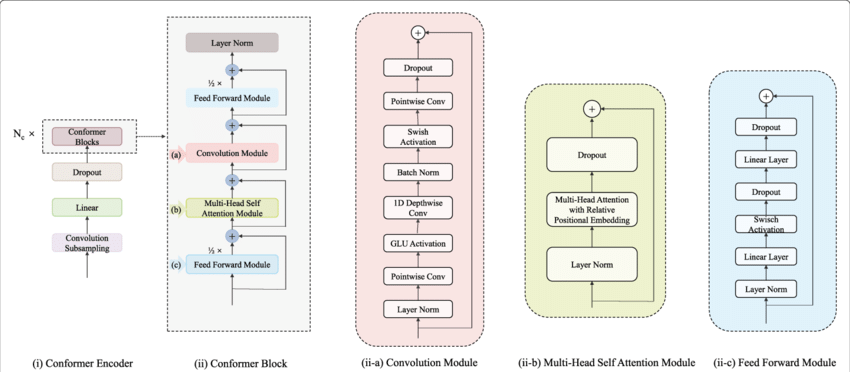
\includegraphics[width=\textwidth,height=0.7\textheight,keepaspectratio]{images/audio-nlp-eval/conformer.png}
    \caption*{\scriptsize Conformer encoder and its sub-modules, after Gulati et al., ``Conformer'', Interspeech 2020, Fig.~1. Redrawn version from Li et al., ``Adversarial joint training with self-attention mechanism for robust end-to-end speech recognition'', EURASIP J.\ Audio Speech Music Process., 2021.}
\end{figure}

\end{frame}

\begin{frame}[allowframebreaks]{Comparing Whisper vs. Conformer}

\begin{itemize}
    \item Whisper and Conformer represent two modern approaches to ASR with complementary strengths:

    \item \textbf{Whisper:}
    \begin{itemize}
        \item Multilingual, trained on a massive weakly supervised dataset.
        \item Robust to accents, noise, and varied conditions.
        \item Open-sourced, general-purpose.
    \end{itemize}

    \item \textbf{Conformer:}
    \begin{itemize}
        \item Efficient hybrid model combining convolution + transformer.
        \item Excels on English benchmarks like LibriSpeech.
        \item Often fine-tuned for specific tasks.
    \end{itemize}
\framebreak
    \item Trade-offs:
    \begin{itemize}
        \item Whisper is more general-purpose, handles diverse languages and noisy conditions.
        \item Conformer achieves very low WER on read English speech ($2.1\%$ on LibriSpeech test-clean without an LM) but may require task-specific tuning.
    \end{itemize}
\end{itemize}

\end{frame}


\begin{frame}[allowframebreaks]{Types of ASR Errors}

\begin{itemize}
    \item Understanding the types of errors in ASR helps diagnose model weaknesses and improve performance.

    \item Common error types:
    \begin{itemize}
        \item \textbf{Substitution:} a word is replaced by another.  
        Example: ``cat'' → ``cap''
        \item \textbf{Deletion:} a word is dropped.  
        Example: ``the cat sat'' → ``cat sat''
        \item \textbf{Insertion:} an extra word is added.  
        Example: ``cat sat'' → ``the cat sat''
    \end{itemize}
\end{itemize}

\end{frame}


\begin{frame}[allowframebreaks]{Factors Affecting ASR Performance}

\begin{itemize}
    \item Several factors influence how well an ASR system performs in real-world conditions:

    \item \textbf{Noise level and microphone quality:}  
    Background noise or poor recording devices can degrade feature extraction and recognition accuracy.

    \item \textbf{Speaker variability:}  
    Differences in accent, pitch, speaking rate, or pronunciation can challenge the acoustic model.

    \item \textbf{Domain mismatch:}  
    Models trained on casual speech may struggle with specialized domains (e.g., medical or legal speech).

    \item \textbf{Training data size and diversity:}  
    More diverse and larger datasets generally improve robustness across speakers, accents, and environments.
\end{itemize}

\end{frame}
